\documentclass[hyperref={pdfpagelabels=false}]{beamer}
\usepackage{lmodern}
\title{Bisphenol-A}   
\author{Jakob Bolenbach} 
\date{\today} 
\setbeamertemplate{navigation symbols}{}
\usepackage{beamerthemeshadow}
\beamersetuncovermixins{\opaqueness<1>{25}}{\opaqueness<2->{15}}
\usepackage{natbib}                  
\usepackage{bibgerm} 

\begin{document}
\begin{frame}
\titlepage
\end{frame} 

\section{Was ist das?} 
\begin{frame}
\frametitle {Was ist das?}
\begin{figure}
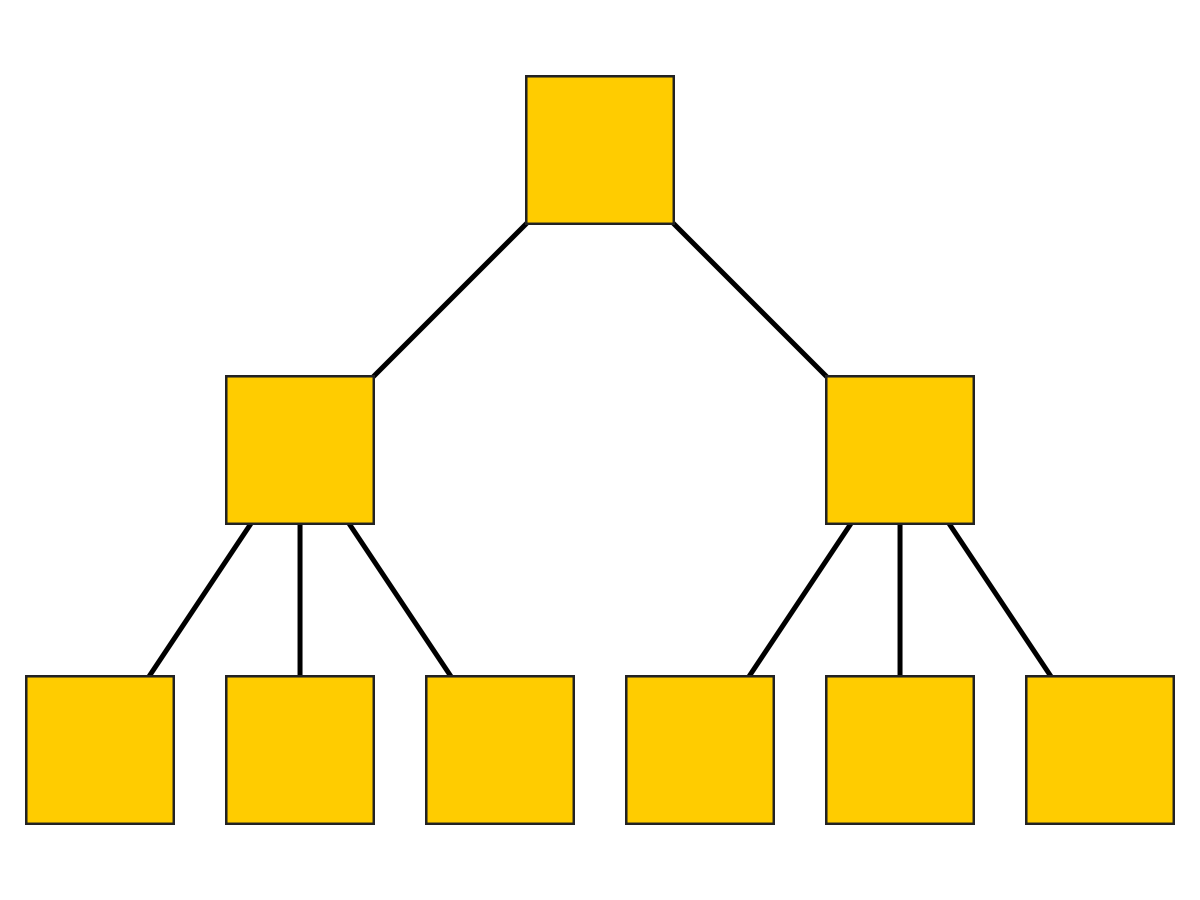
\includegraphics[scale=.2]{HD.png}
\centering
\end{figure}
\end{frame}

\section{Pro und Kontra} 
\begin{frame}
\frametitle{Vorteile}
\begin{itemize}
\item<1-> Einfach
\item<2-> Einfacher Zugriff auf zusammenhängende Strukturen
\item<3-> Schneller Zugriff bei bekannten Pfaden
\end{itemize}
\end{frame}
\begin{frame}
\frametitle{Nachteile}
\begin{itemize}
\item<1-> Unflexibel
\item<2-> Zugriff nur durch die Hierarchie
\item<3-> Keine bidirektionalen Beziehungen 
\end{itemize}
\end{frame}
\section{Quellen}
\begin{frame}
\frametitle{Quellen}
\begin{enumerate} 
\item $https://www.softguide.de/software-tipps/hierarische-datenbanken$
\item $https://en.wikipedia.org/wiki/Hierarchical_database_model$
\end{enumerate}
\end{frame}

\end{document}